%%%%%%%%%%%%%%%%%%%%%%%%%%%%%%%%%%%%%%%%%
% "ModernCV" CV and Cover Letter
% LaTeX Template
% Version 1.11 (19/6/14)
%
% This template has been downloaded from:
% http://www.LaTeXTemplates.com
%
% Original author:
% Xavier Danaux (xdanaux@gmail.com)
%
% License:
% CC BY-NC-SA 3.0 (http://creativecommons.org/licenses/by-nc-sa/3.0/)
%
% Important note:
% This template requires the moderncv.cls and .sty files to be in the same 
% directory as this .tex file. These files provide the resume style and themes 
% used for structuring the document.
%
%%%%%%%%%%%%%%%%%%%%%%%%%%%%%%%%%%%%%%%%%

%----------------------------------------------------------------------------------------
%	PACKAGES AND OTHER DOCUMENT CONFIGURATIONS
%----------------------------------------------------------------------------------------

\documentclass[11pt,a4paper, twoside]{moderncv} % Font sizes: 10, 11, or 12; paper sizes: a4paper, letterpaper, a5paper, legalpaper, executivepaper or landscape; font families: sans or roman
\usepackage[utf8]{inputenc}
\moderncvstyle{classic} % CV theme - options include: 'casual' (default), 'classic', 'oldstyle' and 'banking'
\moderncvcolor{orange} % CV color - options include: 'blue' (default), 'orange', 'green', 'red', 'purple', 'grey' and 'black'
\usepackage{lipsum} % Used for inserting dummy 'Lorem ipsum' text into the template
\usepackage{courier}
\usepackage[scale=0.825]{geometry} % Reduce document margins
%\setlength{\hintscolumnwidth}{3cm} % Uncomment to change the width of the dates column
%\setlength{\makecvtitlenamewidth}{10cm} % For the 'classic' style, uncomment to adjust the width of the space allocated to your name
\usepackage[export]{adjustbox}

\usepackage{setspace}
\setstretch{1.3}
%----------------------------------------------------------------------------------------
%	NAME AND CONTACT INFORMATION SECTION
%----------------------------------------------------------------------------------------

\firstname{Zhijian} % Your first name
\familyname{Wen} % Your last name

% All information in this block is optional, comment out any lines you don't need
\title{Curriculum Vitae}
\address{Unit 304, 20 Upper Queen Street}{Auckland}
\mobile{021-0799395}


\email{zhijianwen1992@gmail.com}
% \homepage{alannungaray.com.mx/}{alannungaray.com.mx} % The first argument is the url for the clickable link, the second argument is the url displayed in the template - this allows special characters to be displayed such as the tilde in this example
% \extrainfo{https://www.facebook.com/AlanDNungaray}
% \photo[60pt][0.4pt]{pictures/foto} % The first bracket is the picture height, the second is the thickness of the frame around the picture (0pt for no frame)

%----------------------------------------------------------------------------------------

\begin{document}

\makecvtitle % Print the CV title

%----------------------------------------------------------------------------------------
%	EDUCATION SECTION
%----------------------------------------------------------------------------------------

\section{Personal Summary}
I am a graduate with Master major in Statistics, with experiences in data analysis/modeling,
programming including developing R-package and data mining. I am interested in programming and I am enjoying to “talk” with computers. I wish to learn more programming in my future. I am keen to join your company where I want
to utilize my skills in creative. \\

\section{Education}
\cventry{2016--2017}{Msc - Statistics}{University of Auckland}{}{}{
	\textit{Key course: Multivariate Analysis, Data Science Practice, Statistical Inference} \\
	\textit{Master of Science with First Class Honours}
}
	
\cventry{2015--2016}{BSc(Hons) - Statistics}{University of Auckland}{}{}{
	\textit{Key course: Bayesian Inference, Statistical Computing, Statistical Modelling}\\
	\textit{class representation of \textbf{Stats 779} }
}
\cventry{2012--2015}{BSc - Mathematics and Statistics}{University of Auckland}{}{}{
	\textit{Key course: Data Technologies, Applied Multivariate Analysis}
	}

\section{Projects}
\cventry{Master \\ 
		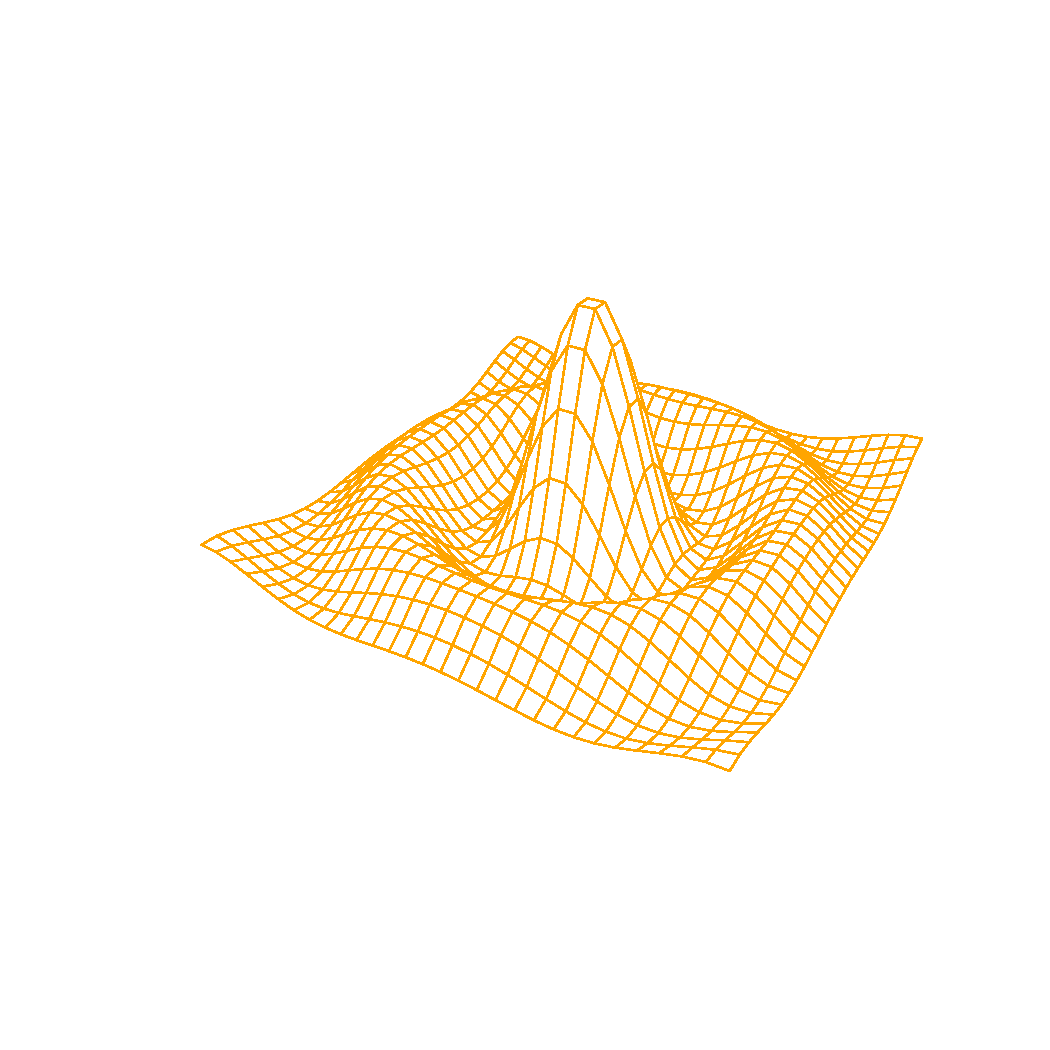
\includegraphics[height = 2.6cm]{persp.pdf}
	}{Emulate the \texttt{persp} plot and \texttt{filled.contour} plot in \texttt{gridGraphics}}{}{}{}{
		\textit{
			The core graphics system in \textbf{R} can be divided into two main packages, the older package called \textbf{graphics} and the newer package called \textbf{grid}. \\
			The \texttt{persp()} is used for drawing 3-D surface and the \texttt{filled.contour()} is used for
			drawing filled level contours in the \textbf{graphics}-package. The aim of this project is to implement these two kinds of plots on the \textbf{grid}-package. \\
			Supervisor: Associate Professor Paul Murrell}
}
\cventry{Honours}{Bayesian inference on forensic glass evidence}{}{}{}{
		\textit{If a person breaks glass, the tiny broken fragments will transfer to the person. If the glass is broken during the commission of the crime, then these tiny fragments can be used as forensic evidence. \\
			The aim of this project is to fit a zero inflated Poisson mixture model and zero inflated negative mixture model under different situations (e.g. The breaker's distance from the window, Proportion of high persistence fragments)}. \\
		\textit{Supervisor: Professor James Curran} \\
}


\section{Work Experience}
% Arguments not required can be left empty
\cventry{2016-Present}{Teaching assistant}  {University of Auckland}{}{}{
	~\\
	\textbf{Tutor of Stats 210}: This course introduces the theory that underlies the statistical methods used in practical statistics courses. My job is:
		\begin{itemize}
			\item To help students to understand the concepts of the course
			\item To help students to solve the problems of tutorials and workshops. \\
		\end{itemize}	
	\textbf{Tutor and Marker of Stats 220}: This course introduces a variety of computer technologies relevant to storing, managing, and processing data. My job is to help students to understand and solve the ``technical'' problems:
		\begin{itemize}
			\item The World-Wide Web (HTML), Data Description (XML)
			\item Data Storage (Spreadsheets, Databases), Data Management and Queries (SQL)
			\item Data Processing (Scripting, Pattern Matching, R) \\
		\end{itemize}
	\textbf{Marker of Stats 380}: A course of statistical computing using the \texttt{R} statistical computing environment\\}

\cventry{2015-2016}{Summer Scholarship}  {University of Auckland}{}{}{
	Working on the \texttt{iNZightMaps}-package, used in the mapping module for \textbf{iNZight} I am one of the authors of the \texttt{iNZightMaps}-package. The works that I have done as follows:
	\begin{itemize}
		\item Map Creation, request a topographic map from Google Maps' API
		\item Visualization of the geographical data. For example, the size of the data points are determined by Magnitude of the earth quakes.
		\item Map Creation, draw the map by using the geographic information system (GIS)
		\item Visualization of the geographical data. For example, the colors of the counties are determined by the ratio of the Population ratio.
	\end{itemize}
}




%------------------------------------------------
%----------------------------------------------------------------------------------------
%	AWARDS SECTION
%----------------------------------------------------------------------------------------

%----------------------------------------------------------------------------------------
%	COMPUTER SKILLS SECTION
%----------------------------------------------------------------------------------------

\section{Skills}

\cvitem{Advance:}{\textsc{R}, \textsc{HTML}, \LaTeX} 
\cvitem{Fair:}{SAS, SQL, jags, Linux, Lua, JavaScript, GitHub}
\cvitem{Basic:}{C, C++, JAON, XML, \textsc{Matlab}, Excel}


%----------------------------------------------------------------------------------------
%	LANGUAGES SECTION
%----------------------------------------------------------------------------------------

\section{Languages}
\cvitemwithcomment{}{English, Mandarin, Cantonese}{}


%----------------------------------------------------------------------------------------
%	INTERESTS SECTION
%----------------------------------------------------------------------------------------
\section{Interest}
\cvlistdoubleitem{Game Computing}{Statistical Computing}
\cvlistdoubleitem{Table tennis}{Physics}


%----------------------------------------------------------------------------------------
%	Reference SECTION
%----------------------------------------------------------------------------------------
\section{Reference}
\cvitem{}{Avaiable upon request
}  {}


%----------------------------------------------------------------------------------------
%	COVER LETTER
%----------------------------------------------------------------------------------------

% To remove the cover letter, comment out this entire block



%----------------------------------------------------------------------------------------

\end{document}